\section{Analiza konkurencyjnych rozwiązań}

\phantom{Th}

Na rynku znajduje się wiele narzędzi do organizacji czasu, ale \textbf{kalendarz Google} pozostaje niekwestionowanym liderem.
Jest to profesjonalne i przede wszystkim darmowe, preinstalowane narzędzie na większości urządzeń z systemem Android.
Według raportu stworzonego przez zespół pracujący dla DataReportal, w Polsce na rok 2023, aż 87\% użytkowników posiada
telefon właśnie z tym systemem
\cite{datareportal}. Aplikacja ta stanowi nieodłączny element funkcjonowania firm, zwłaszcza tych początkujących,
ale nie tylko. Ułatwia harmonogramowanie spotkań, śledzenie projektów i pozwala na zachowanie kontroli nad terminami.
Dużym atutem kalendarza Google jest rozdzielenie zadań i wydarzeń na osobne elementy kalendarza (Rys. \ref{fig:googleCalendar}).\\

\begin{figure}[ht]
  \begin{minipage}{0.4\textwidth}
    \centering
    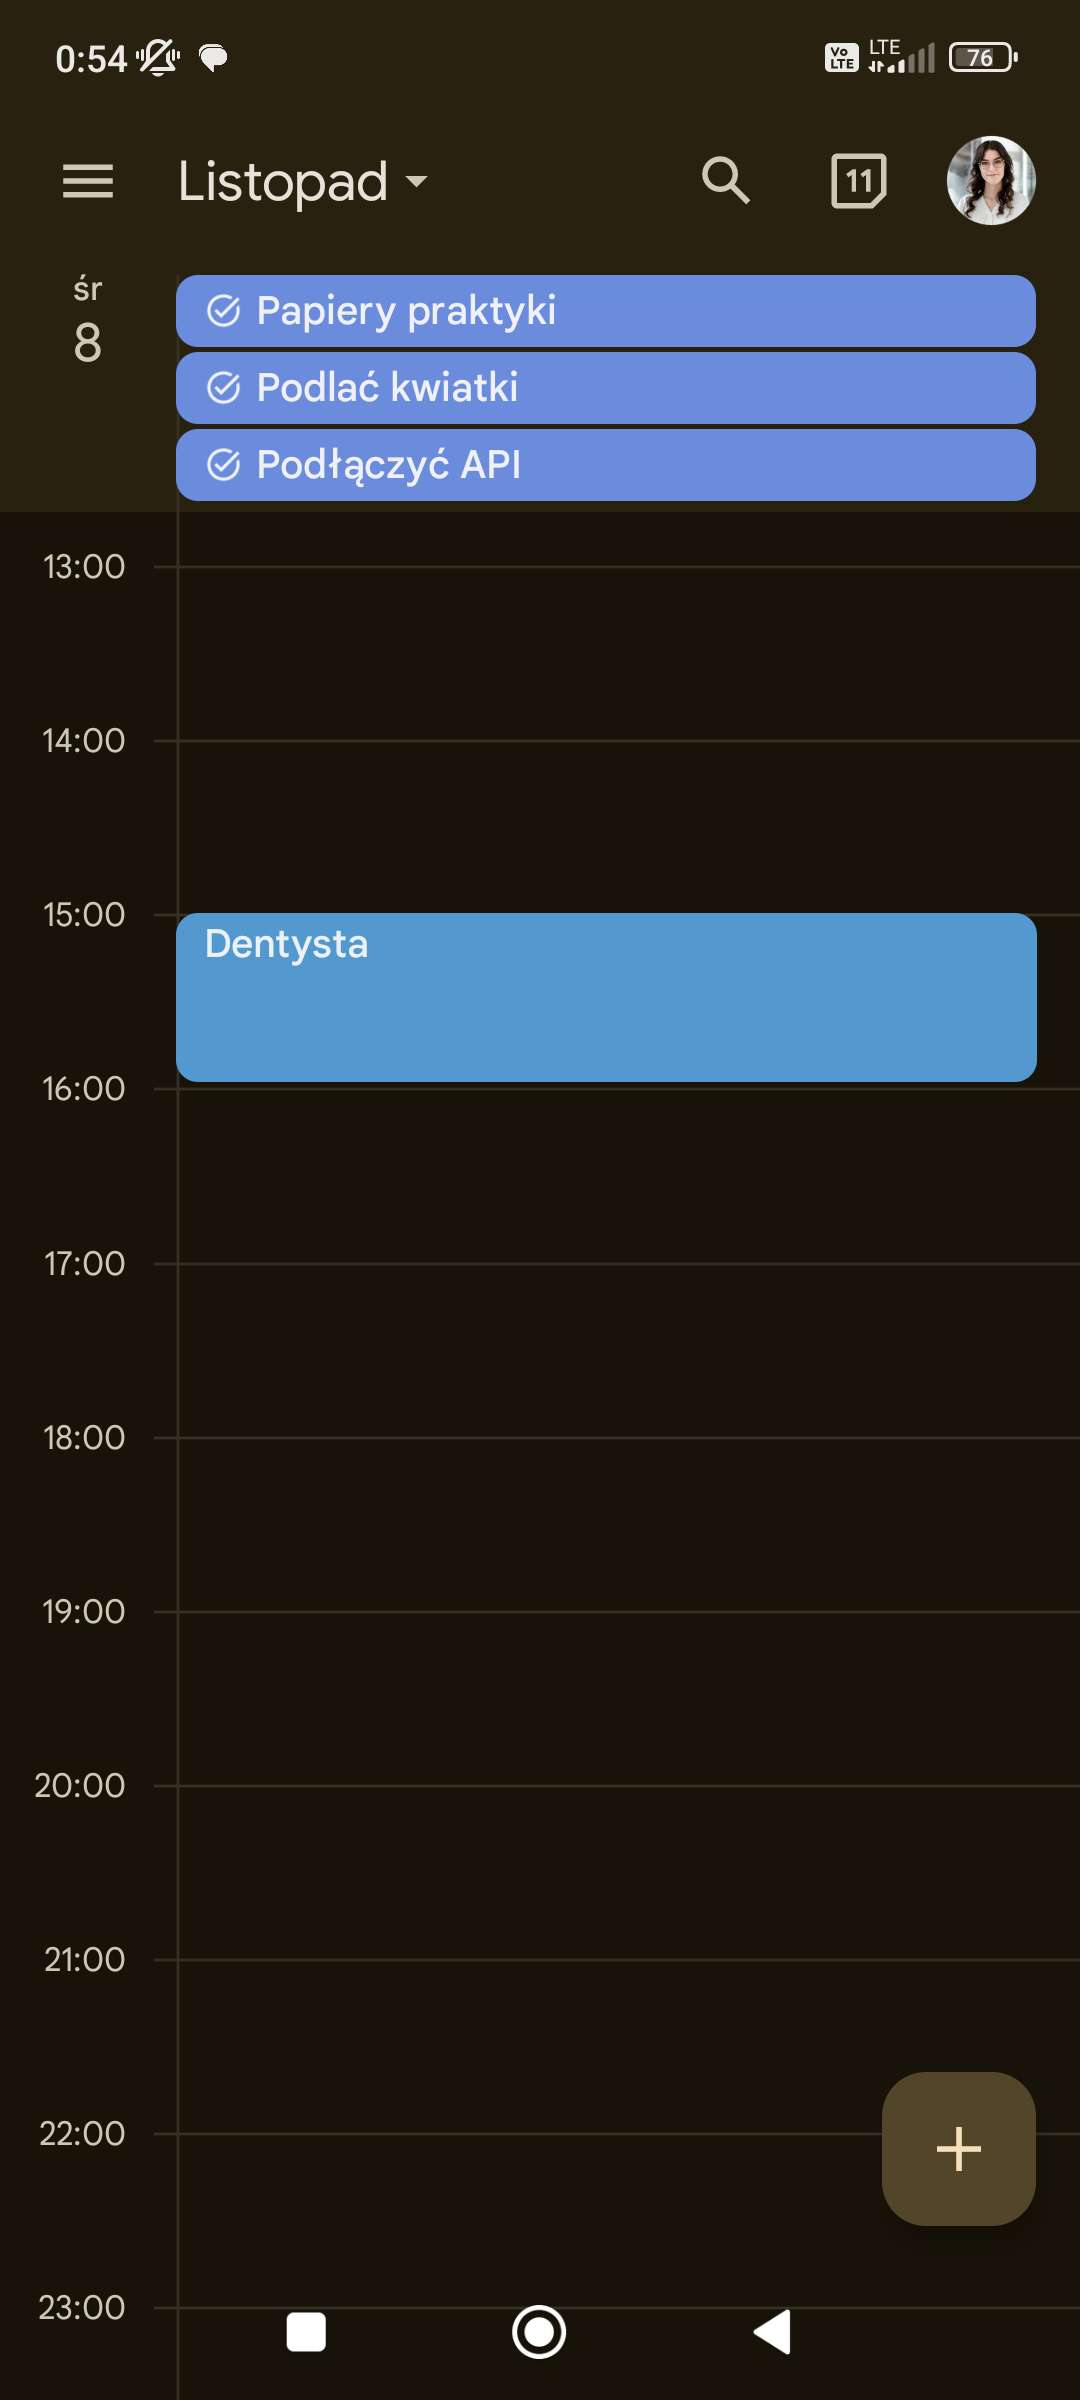
\includegraphics[height=13cm, keepaspectratio]{images/analiza/googleCalendar}
    \caption{Widok konkretnego dnia w kalendarzu Google}
    \label{fig:googleCalendar}
  \end{minipage}
  \hfill
  \begin{minipage}{0.4\textwidth}
    \centering
    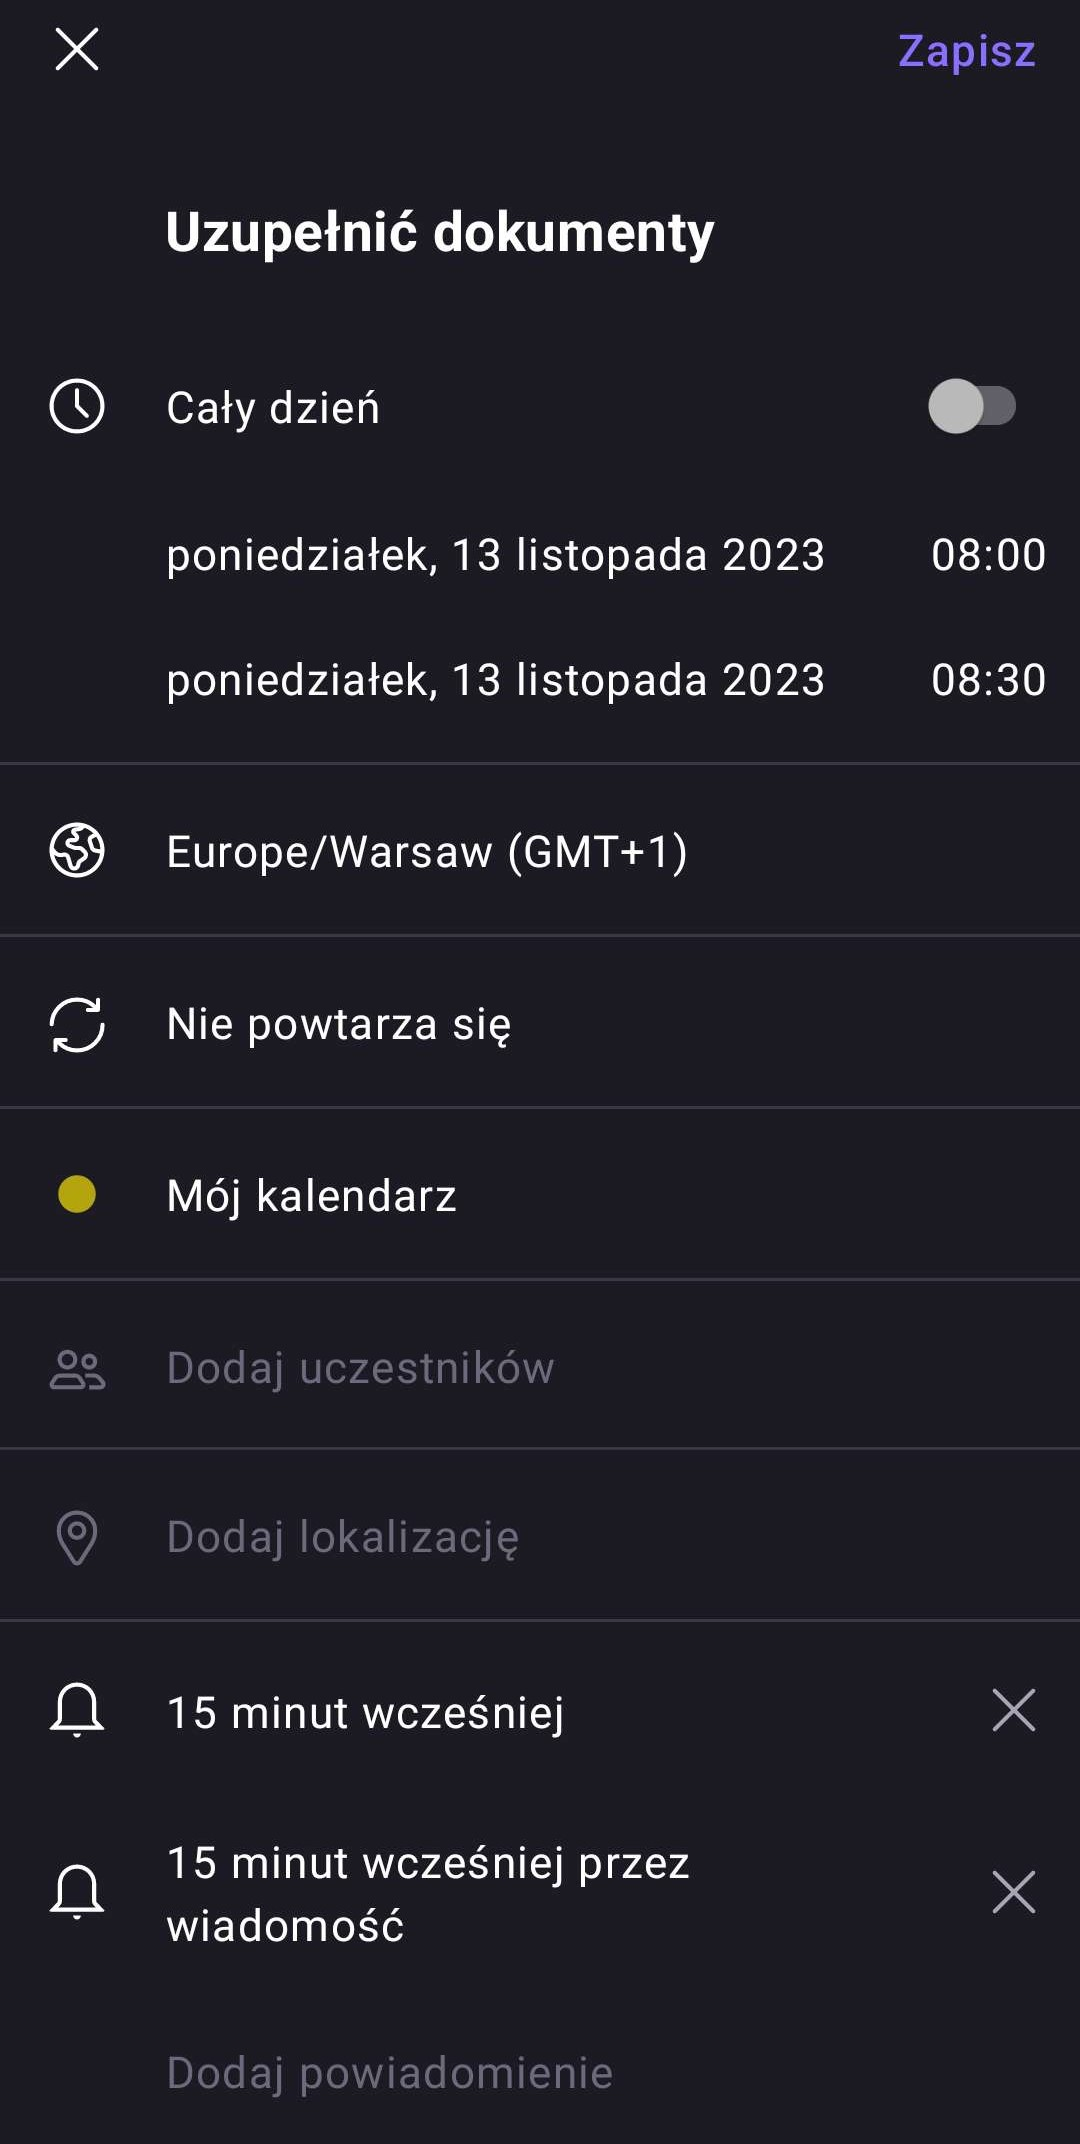
\includegraphics[height=13cm, keepaspectratio]{images/analiza/protonCalendar}
    \caption{Widok tworzenia wydarzenia w kalendarzu Proton}
    \label{fig:protonCalendar}
  \end{minipage}
\end{figure}

Jest to narzędzie umożliwiające precyzyjne określenie wszelkich informacji odnośnie danego wydarzenia.
Nie da się kwestionować, że możliwości jakie daje nam aplikacja są niepotrzebne,
jednakże z punktu widzenia użytkownika końcowego ZodiaCal funkcje takie jak lokalizacja wydarzenia,
link do rozmowy wideo czy określanie trwania każdego jednego wpisanego wydarzenia od do jest zbędne.
W ZodiaCal istotne jest sprawne dodawanie wydarzeń do kalendarza, bez konieczności przeglądania dodatkowych opcji.\\

Dobrą alternatywą dla kalendarza Google jest \textbf{Proton Calendar} (Rys. \ref{fig:protonCalendar}).
Jest to również zaawansowana aplikacja do monitorowania wydarzeń, z tą różnicą,
iż proton specjalizuje się w zapewnianiu jeszcze większej prywatności i bezpieczeństwa użytkowników.
Z tym, że nie rozróżnia wydarzeń od zadań. Proton to firma oferująca usługi związane
z prywatnością online, w tym bezpiecznymi skrzynkami e-mail i kalendarzami.\\


Bardzo ciekawym i minimalistycznym rozwiązaniem jest aplikacja \textbf{135 To Do List} która poprzez swój estetyczny
i prosty interfejs ułatwia użytkownikom priorytetyzacja zadań na konkretny dzień.
Posiada możliwość zmiany kolejności wpisanych już wcześniej zadań oraz widok całego miesiąca.
Niestety nie ma opcji dodawania cyklicznych wydarzeń. ZodiaCal przyświeca niemalże ta sama minimalistyczna
idea tworzenia interfejsu, jednak wprowadza rozbudowane funkcje, takie jak codzienny horoskop i osobisty dziennik pielęgnacji (Rys. \ref{fig:ToDoList}).\\

\textbf{FeelingMySkin} to bardzo rozbudowane narzędzie do precyzyjnego określenia pielęgnacji cery i nie tylko.
Korzystając z niej użytkownik może układać plany pielęgnacyjne z wykorzystaniem konkretnych produktów,
których używa na co dzień, monitorować zmiany skórne, czy chociażby śledzić daty przydatności produktów.
To z pewnością przydatna aplikacja, jednakże wymaga czasu, aby opanować wszystkie możliwe funkcje.
Interfejs strony głównej jest bardzo przeładowany informacjami, co utrudnia korzystanie z aplikacji w sposób efektywny (Rys. \ref{fig:feelingMySkin}).\\

\begin{figure}[ht]
  \begin{minipage}{0.4\textwidth}
    \centering
    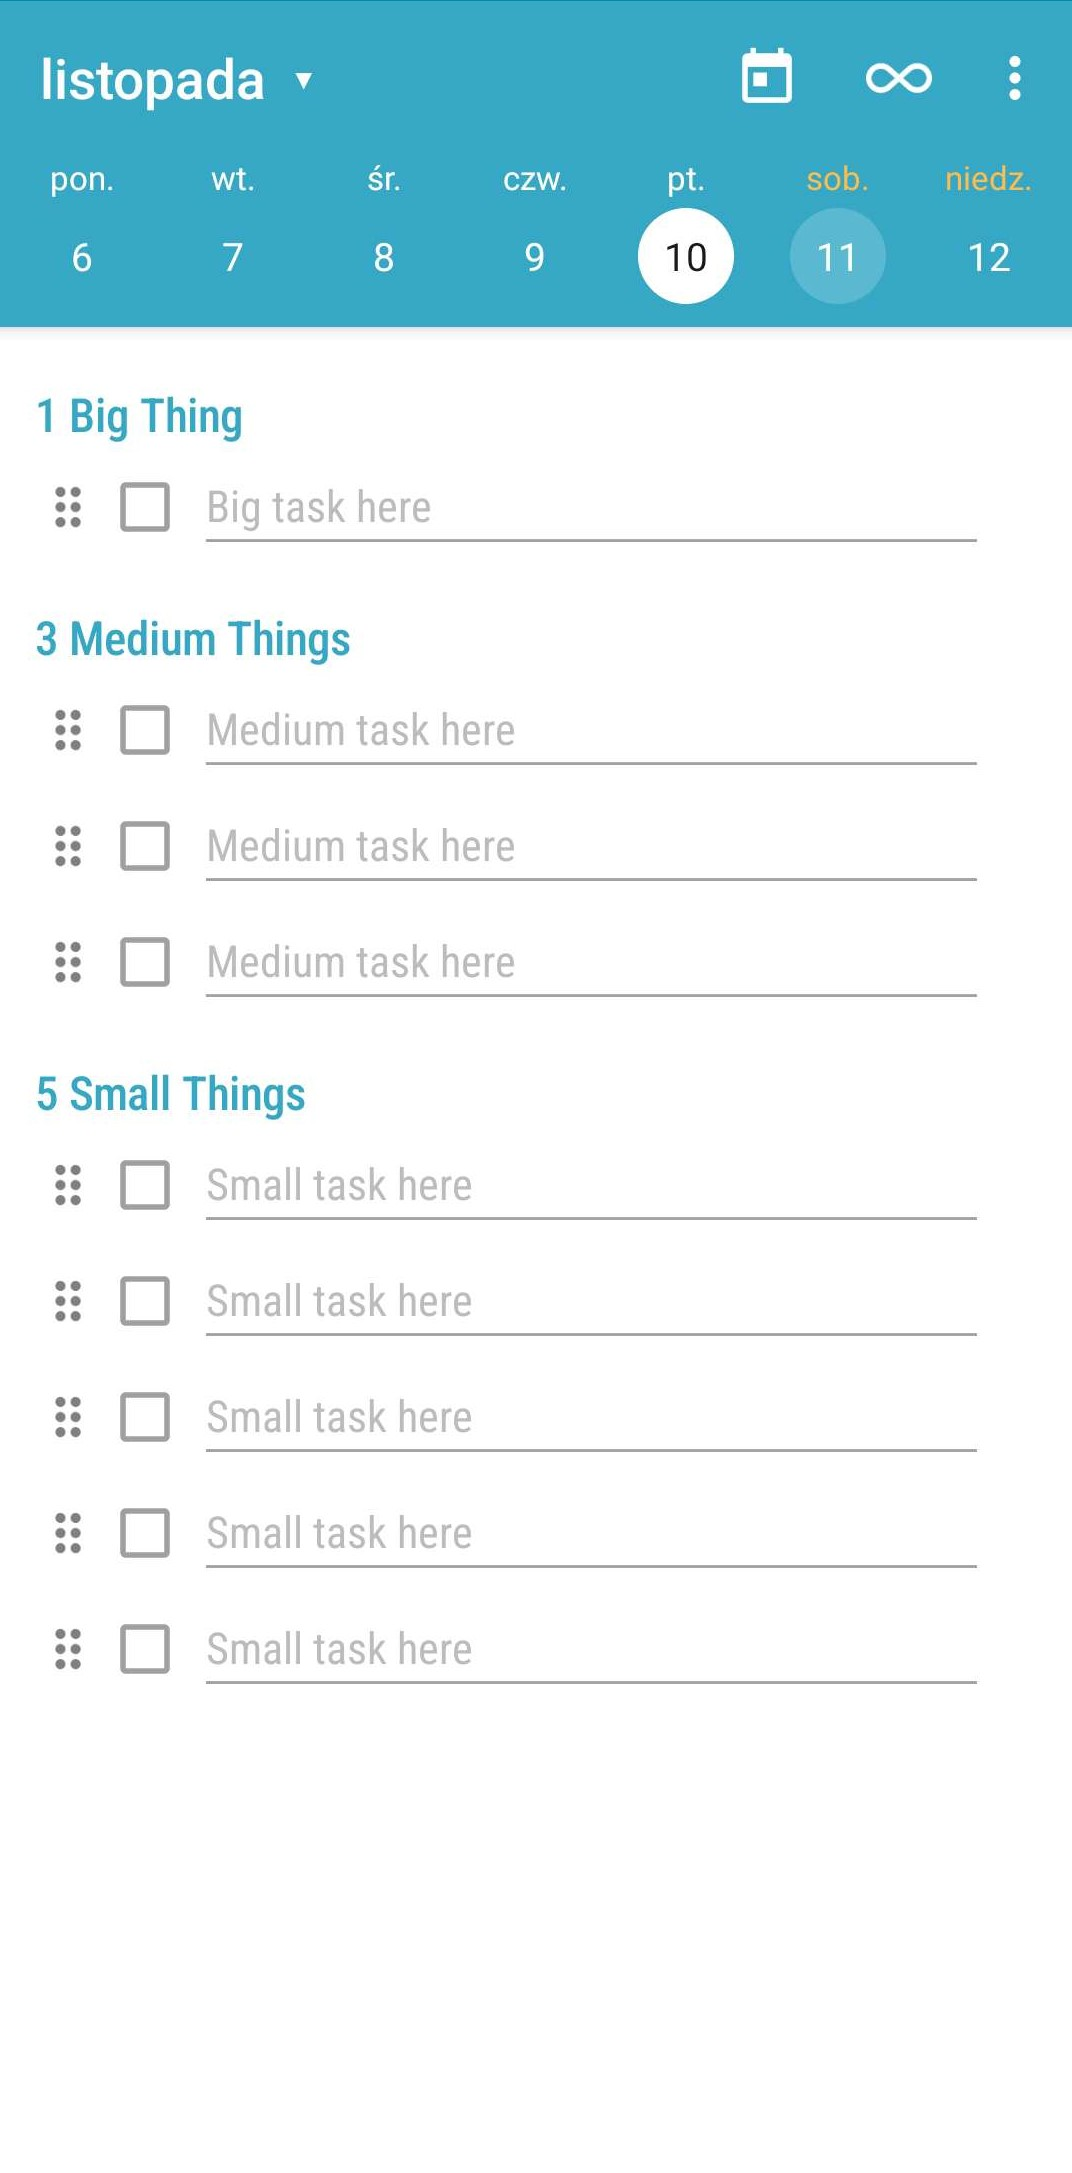
\includegraphics[height=13cm, keepaspectratio]{images/analiza/135ToDoList}
    \caption{Ekran główny aplikacji 135 To Do List}
    \label{fig:ToDoList}
  \end{minipage}
  \hfill
  \begin{minipage}{0.4\textwidth}
    \centering
    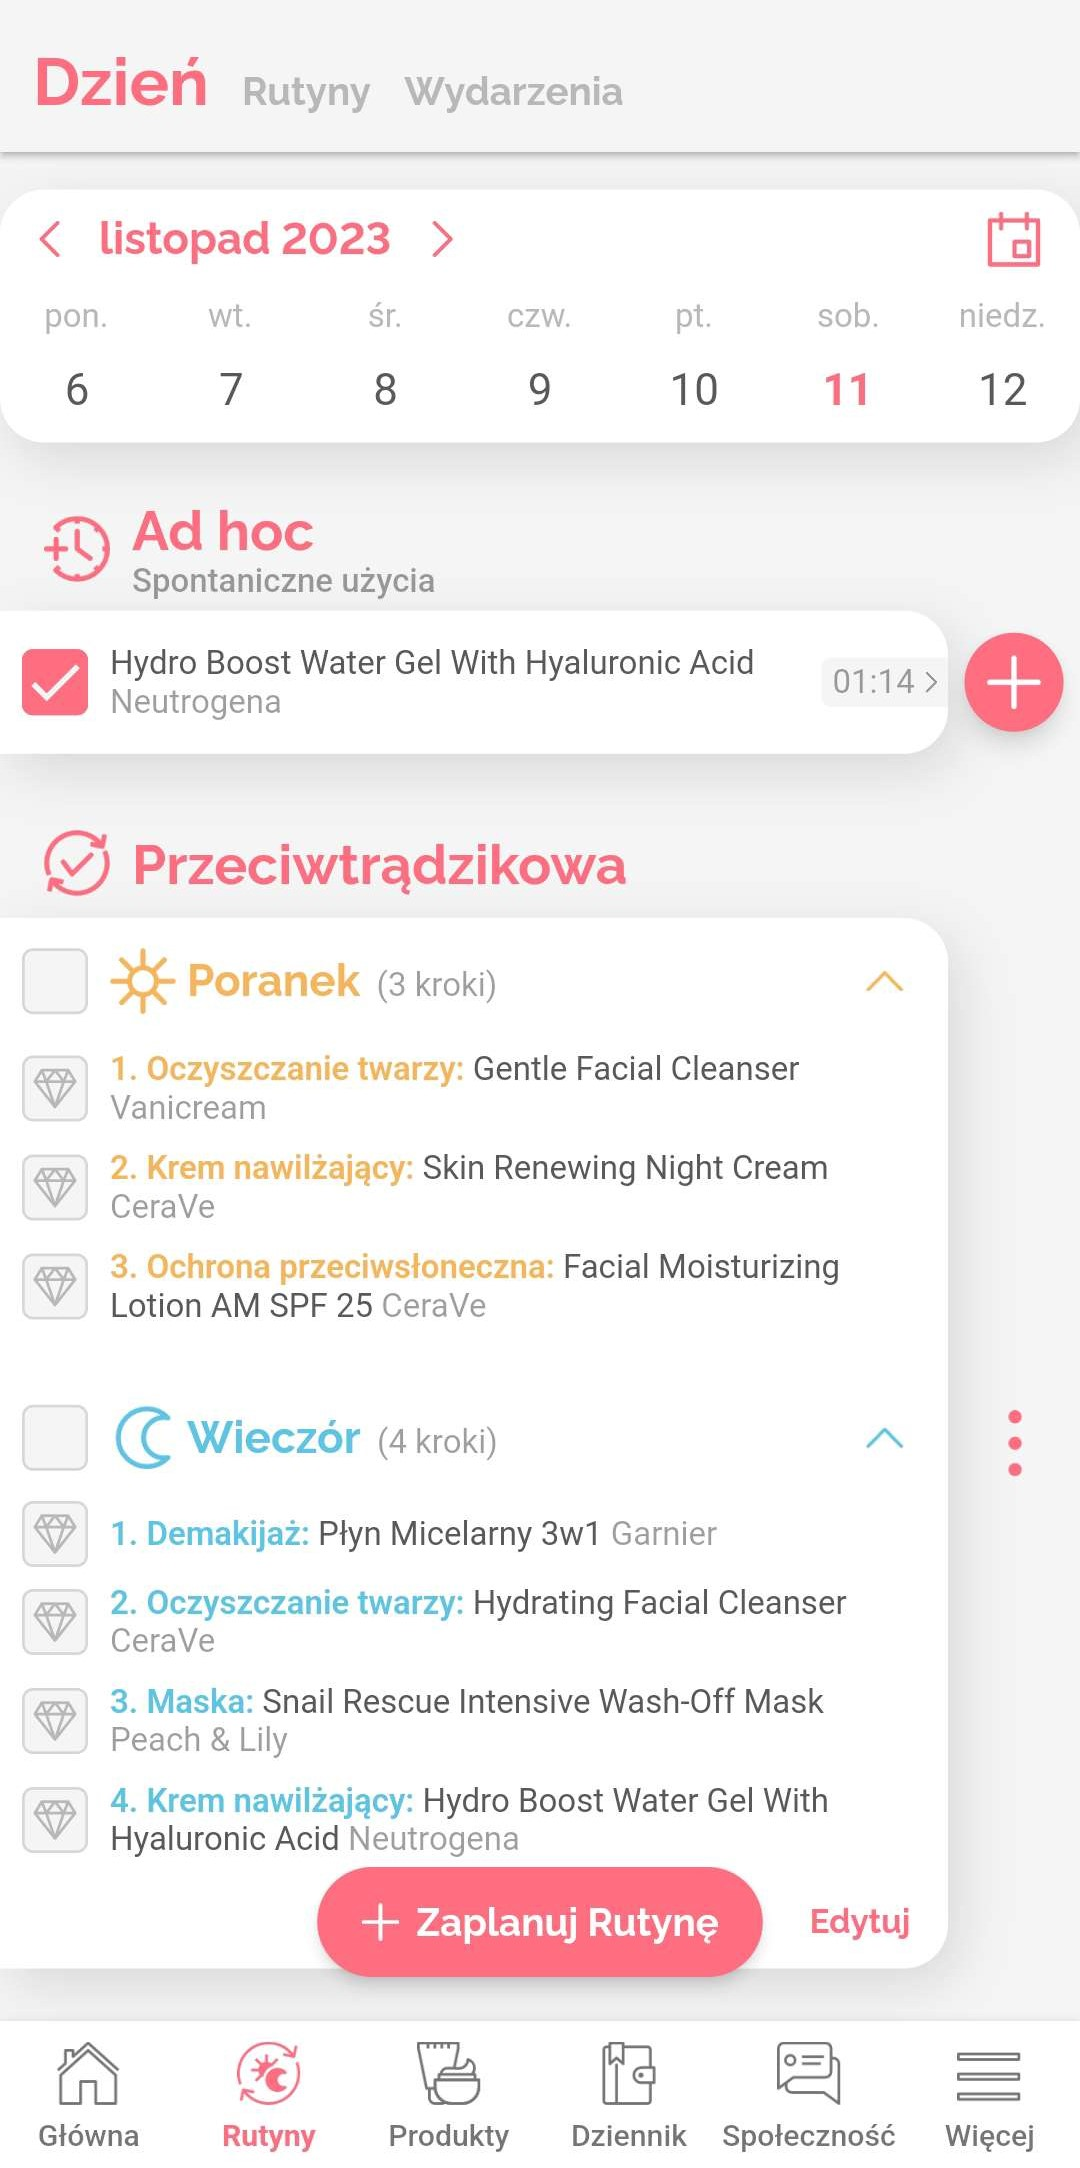
\includegraphics[height=13cm, keepaspectratio]{images/analiza/feelingMySkin}
    \caption{Widok codziennej rutyny w aplikacji FeelingMySkin}
    \label{fig:feelingMySkin}
  \end{minipage}
\end{figure}

ZodiaCal to hybryda wszystkich wymienionych aplikacji.
To minimalistyczne narzędzie służące do wielu celów, ale w podstawowym zakresie.
Próbuje połączyć najlepsze cechy różnych istniejących aplikacji,
oferując minimalistyczny interfejs do zarządzania czasem, zadaniami i nie tylko.
Chociaż nie zawiera wszystkich zaawansowanych funkcji dostępnych w innych aplikacjach,
dąży do dostarczenia użytkownikom wyważonego narzędzia do pracy.


\section{Analiza SWOT}
\phantom{Th}
Analiza SWOT to termin powstały od pierwszych liter poszczególnych słów w języku angielskim,
czyli Strengths - siły, Weaknesses - słabości, Opportunities - szanse oraz Threats - zagrożenia.
Jest to metoda analizy rynku, która cieszy się popularnością wśród współczesnych przedsiębiorców.
Takie podejściu do projektu pozwala na lepsze zrozumienie wpływów istniejących już warunków na przyszłość,
szybkie określenie planów strategicznych oraz ułatwia podejmowania decyzji.
Cieszy się popularnością ze względu na prostotę oraz skuteczność działania \cite{businessanalysis}.



\subsubsection*{\textbf{Mocne strony (Strengths):}}
\phantom{Th}
Czynniki aplikacji, które podnoszą jej przewagę konkurencyjną. W tej chwili rynek rozdziela kalendarz osobisty i dzienniczek pielęgnacji na dwie różne aplikację,
co prowadzi do tego, że użytkownik nie tylko musi uzupełniać pola w dwóch różnych miejscach,
uczyć się dwóch różnych interfejsów, ale również przekazywać swoje dane do dwóch różnych serwisów.
Interfejsy wymienionych aplikacji posiadają wiele funkcji do precyzyjnego określania zadań
czy pielęgnacji przez co opanowanie ich zajmuje więcej czasu i wysiłku użytkownika,
niż gdyby posiadały jedynie podstawowe funkcje w tym zakresie.
Aplikacja została stworzona z myślą o wielu platformach dzięki czemu może dotrzeć do szerszej grupy odbiorców.
Opcja, której nie spotkamy w żadnym innym kalendarzu to możliwość sprawdzenia codziennego horoskopu dostosowanego do znaku zodiaku użytkownika.
Dodatkowo, jeśli użytkowni nie wie w jaki sposób określić swój znak zodiaku, aplikacji zrobi to za niego, wystarczy podać dzień i miesiąc urodzenia.


\subsubsection*{\textbf{Słabe strony (Weaknesses):}}
\phantom{Th}
Czynniki aplikacji, które osłabiają jej pozycję. Prostota jest jednocześnie zaletą i wadą. Wadą, ponieważ może nie spełniać oczekiwań zaawansowanych użytkowników,
którym może brakować pewnych funkcji. Brak bazy danych produktów to kolejna słabość projektu.
W aplikacji nie ma możliwości wybrania z bazy danych kosmetyków, których użytkownik używa podczas pielęgnacji jak to mam miejsce w FeelingMySkin.
Opcja ta jest nie dostępna, ponieważ wiązałaby się z podpięciem do przekraczającej wielkościami bazy danych
oraz nieustanne aktualizowanie jej za każdym nowym wprowadzonym produktem na rynek.
Innym negatywnym aspektem jest fakt, iż obecnie rynek przepełniony jest aplikacjami o podobnym charakterze.
W związku z tym konieczne może być przeprowadzenie skutecznej kampanii reklamowej, aby wyróżnić aplikację wśród konkurencji.


\subsubsection*{\textbf{Szanse (Opportunities):}}
\phantom{Th}
Czynniki zewnętrzne, które mają pozytywny wpływ na obecną sytuację na rynku. Ostatnio obserwuje się rosnące zainteresowanie świadomą pielęgnacją skóry,
co przekłada się na wzrost zapotrzebowania na aplikacje ułatwiające planowanie pielęgnacji, czy monitorowanie stanów skóry.


\subsubsection*{\textbf{Zagrożenia (Threats):}}
\phantom{Th}
Czynniki zewnętrzne, które mogą negatywnie wpłynąć na aplikację. Największym wyzwaniem jest zagwarantowanie prywatności i bezpieczeństwa danych.
Konieczne jest zapewnienie wysokiego poziomu ochrony danych użytkowników, zwłaszcza w obszarze związanym z informacjami o pielęgnacji skóry,
które uważane są za dane wrażliwe. Następnym wadliwym punktem są zmiany w regulacjach dotyczących prywatności w różnych państwach.
Zmiany przepisów dotyczących ochrony danych osobowych mogą wymagać dostosowania polityki prywatności aplikacji,
w związku z tym, istotne jest, aby systematycznie monitorować ewentualne zmiany w przepisach.


\section{Analiza przedmiotowa MoSCoW}
\phantom{Th}
Analiza MoSCoW podobnie jak analiza SWOT jest akronimem. Dzieli wymagania na cztery kategorię, uwzględniające wzrastającą złożoność. 
Są to kolejno M (Must have) wymagania konieczne, S (Should have) wymagania wskazane, C (Could have) wymagania opcjonalne, 
W (Won't have) wymagania wykluczone. Metoda ta pomaga w ustaleniu priorytetów, które w sposób uzasadniony zapewnia kompletny 
i dokładny zestaw wymagań, które aplikacja musi spełnić. Takie podejście uświadamia, które funkcje są niezbędne do funkcjonowania systemu 
i zapobiega realizacji zadań opcjonalnych przed ukończeniem zadań obowiązkowych \cite{moscow} , \cite{businessanalysis}. 

\subsubsection*{\textbf{Must have}}
\phantom{Th}
Zbiór funkcji oznaczony jako Must have to kategorie wymagań, które system jest zobowiązany posiadać. 
Podstawowym elementem aplikacji jest połączenie z bazą danych, którą należy w pierwszej kolejności skonfigurować
i podłączyć. Konieczne jest utworzenie modelu danych oraz zapewnienie niezbędnych operacji, 
które umożliwią efektywne zarządzanie danymi użytkowników w systemie. Aby korzystać z aplikacji potrzebne jest konto, 
co oznacza, że niezbędnym elementem jest ekran logowania i rejestracji. 
Ponadto ekrany te muszą posiadać walidację formularzy przed wysłaniem ich na serwer. Zapewni to poprawność 
i integralność danych wprowadzanych przez użytkowników oraz pomoże uniknąć potencjalnych błędów 
i problemów związanych z danymi przechowywanymi w systemie.\\

Drugim fundamentem aplikacji jest funkcja kalendarza. Musi ona zapewniać możliwość dodawania, usuwania oraz edytowania wydarzeń, zadań. 
Dodatkowo ważnym aspektem jest widok kalendarza na cały rok, miesiąc, tydzień i dzień. 
Niezbędną funkcją jest również możliwość rejestrowania swojej pielęgnacji na dany dzień, w zależności od kategorii nawilżanie, 
złuszczanie, odbudowa, przerwa. Kolejną kluczową funkcją jest wyświetlanie horoskopu dla znaku zodiaku użytkownika, 
co wiąże się ze znalezieniem odpowiedniego API oraz połączenia go z aplikacją.


\subsubsection*{\textbf{Should have}}
\phantom{Th}
W kontekście sekcji Should have skupiamy się na wymaganiach, które są ważne, ale nie są absolutnie niezbędne dla funkcjonowania systemu. 
Przydatną funkcją związaną z kalendarzem, z perspektywy użytkownika końcowego jest możliwość automatycznego uzupełnianie pól cyklicznych 
takich jak praca/studia oraz otrzymywanie powiadomień. Z kolei rozszerzeniem funkcji pielęgnacji jest opcja związana z dodawaniem 
produktów do danej pielęgnacji. Natomiast rozbudowaniem modułu horoskopu jest funkcja przydzielania znaku zodiaku 
z podanej daty przez użytkownika. Wiele aplikacji umożliwia logowanie się za pomocą kont z mediów społecznościowych, 
dlatego warto dodać opcję logowania się przy użyciu konta Google, aby sprostać obowiązującym standardom. 

\subsubsection*{\textbf{Could have}}
\phantom{Th}
Funkcje w grupie Could have to wymagania, które dobrze jest mieć, ale nie są kluczowe. 
Dobrym obszarem do rozbudowy jest moduł związany z pielęgnacją. 
Można rozszerzyć go o wyświetlaniu wykresów pod koniec miesiąca, 
monitorowanie daty ważności używanych produktów oraz dodanie Trackerów samopoczucia, snu i nawyków. 
Tracker to narzędzie pozwalające na odnotowanie aktywności w danym stopniu na konkretny dzień. 
Na pewno dużym ułatwieniem dal użytkownika byłoby wprowadzenie możliwości zmiany języka oraz onboardingu zaraz po zarejestrowaniu konta.


\subsubsection*{\textbf{Won't have}}
\phantom{Th}
Wymagania w grupie Won't have mają najniższy priorytet. Określają funkcję, które w tej wersji nie zostaną dostarczone, 
ale będą zawarte w kolejnej aktualizacji. Klienci często lubią edytować podstawowy interfejs pod siebie, 
więc wprowadzenie personalizacji motywów na pewno korzystnie wpłynęłaby na odbiór aplikacji. 
Dodatkowo coraz więcej użytkowników decyduje się na smatwach'e. 
Przyszłościowym krokiem byłoby umożliwienie korzystania z aplikacji również na zegarku.